% \documentclass[12pt, oneside]{article}
\documentclass[onecolumn]{IEEEtran}
\usepackage[
backend=biber,
style=numeric,
]{biblatex}
\usepackage[utf8]{inputenc}
\usepackage{graphicx}
\graphicspath{ {images/} }
\usepackage{caption}
\usepackage{subcaption}
\usepackage{xcolor}
\usepackage{gensymb}
\usepackage[a4paper, width=150mm, top=25mm, bottom=25mm]{geometry}
% \usepackage[backend=biber]{biblatex}
% \usepackage[backend=biber, style=numeric, sorting=none]{biblatex}
\addbibresource{references.bib}


\begin{document}

\begin{titlepage}
	\begin{center}
	
	\vspace*{0.5cm}
	
	\Huge
	\textbf{Literature Review}
	
	\vspace{0.5cm}
	\Large
	An Analysis of Active Inference and Reinforcement Learning Paradigms in Partially Observable Environments.
	
	\vspace{1.5cm}

	\textbf{Fraser Paterson}

	\vspace{1.5cm}

	A review of the extant literature, pursuant to the requirements of the\\ 
	Degree: Bachelor of Science (Honours).  
	
	\vspace{2.0cm}

	
\includegraphics[width=0.4\textwidth]{UWA_Logo.png}
	
	\vspace{2.0cm}	
	
	\Large
	Supervisor: Dr Tim French\\ 
	Department of Computer Science and Software Engineering\\
	The University of Western Australia\\
	24 April 2023
	\end{center}
\end{titlepage}


\tableofcontents

\cleardoublepage

\section{Overview}
This section should be an overview of the Lit review. Can possibly put some information related to the project in here.

\section{Introduction}

\subsection{Active Inference: An Overview}

Active Inference is an emerging first-principles account of adaptive behavior. Originating from Neuroscience: \textcite{A_FEP_For_The_Brain}, \textcite{The-Bayesian-Brain} and \textcite{Action-Behaviour-FE}, though the theory is increasingly making inroads into Machine Learning and Artificial Intelligence: \textcite{RL-or-AIF} and \textcite{Applications-of-FEP-Machine-Learning-Neuroscience}. Active inference is a highly ambitious theory, as it purports to offer a fully unified account of action, perception and learning: \textcite{FEP-Unified-Brain-Theory}. The basic postulate of the theory is that adaptive systems like living organisms, will act to fulfill prior expectations or ``preferences'' which encode desirable states for that system. The system uses a probabilistic generative model to perform free-energy minimization on a functional of Bayesian beliefs to select actions which will counteract the thermodynamic dispersal of its internal states, away from its ``preferred'' states, thus preserving the system's self-organization. Free-energy may hence be thought of as encoding the ``surprisal'' of a particular sensory observation, given the agent's generative model.

This drive to reduce sensory surpirsal has the effect of introducing an imperative for information-gain in addition to the imperative to maximize reward or ``value''. value maximization is typically the only imperative of interest in more traditional approaches to adaptive behavior, such as Reinforcement Learning; \textcite{Reinforcement-Learning-An-Introduction}. In a nutshell, Active Inference replaces value functions with variational free energy functionals of Bayesian beliefs. Active Inference agents therefore have a built-in affordance for dynamically trading-off pragmatic and epistemic imperatives. 

Historically speaking, Active Inference is a derivative of the ``Free Energy Principle'', which is a theoretical principle thought to plausibly offer a unified, constitutive account of brain function: \textcite{FEP-Rough-Guide-Brain} and perhaps even of life itself: \textcite{Life-As-We-Know-It}. The Free Energy Principle (FEP) attempts to provide a principled account of adaptivity per-se. The basic insight is that if a system maintains a boundary between itself and some exterior environment, and if this system persists over time, then this system must be capable of resisting the thermodynamic tendency toward the dissolution of the boundary which separates its internal states from the external environment. To do this, the system must maintain the configuration of its internal states so as to exist within some desired homeostatic bounds. The way the system can achieve this is by maximizing the Bayesian model-evidence for its configuration of internal states. Hence we have internal states, external states and ``blanket'' states, where the blanket states are themselves composed of ``active'' and ``sensory'' states. Internal states can only be directly influenced by the sensory states of the blanket, and external states can only be influenced by the active states of the blanket. The Bayesian model evidence for the system's configuration of internal states is bounded above by the free energy of the system's Bayesian beliefs about the sensory states. Hence the ``Free Energy'' principle, since the Free Energy serves as a tractable upper bound to the system's model evidence. Thus the principle culminates in the following statement. Any system which persists across time, in the face of a tendency to thermodynamic dissolution must act as if it is soliciting evidence for its own existence, via a model of the world.  

See Figure \ref{fig:FEP} for a diagrammatic exposition of the relationship between these variables.

\begin{figure}[h]
  \centering
  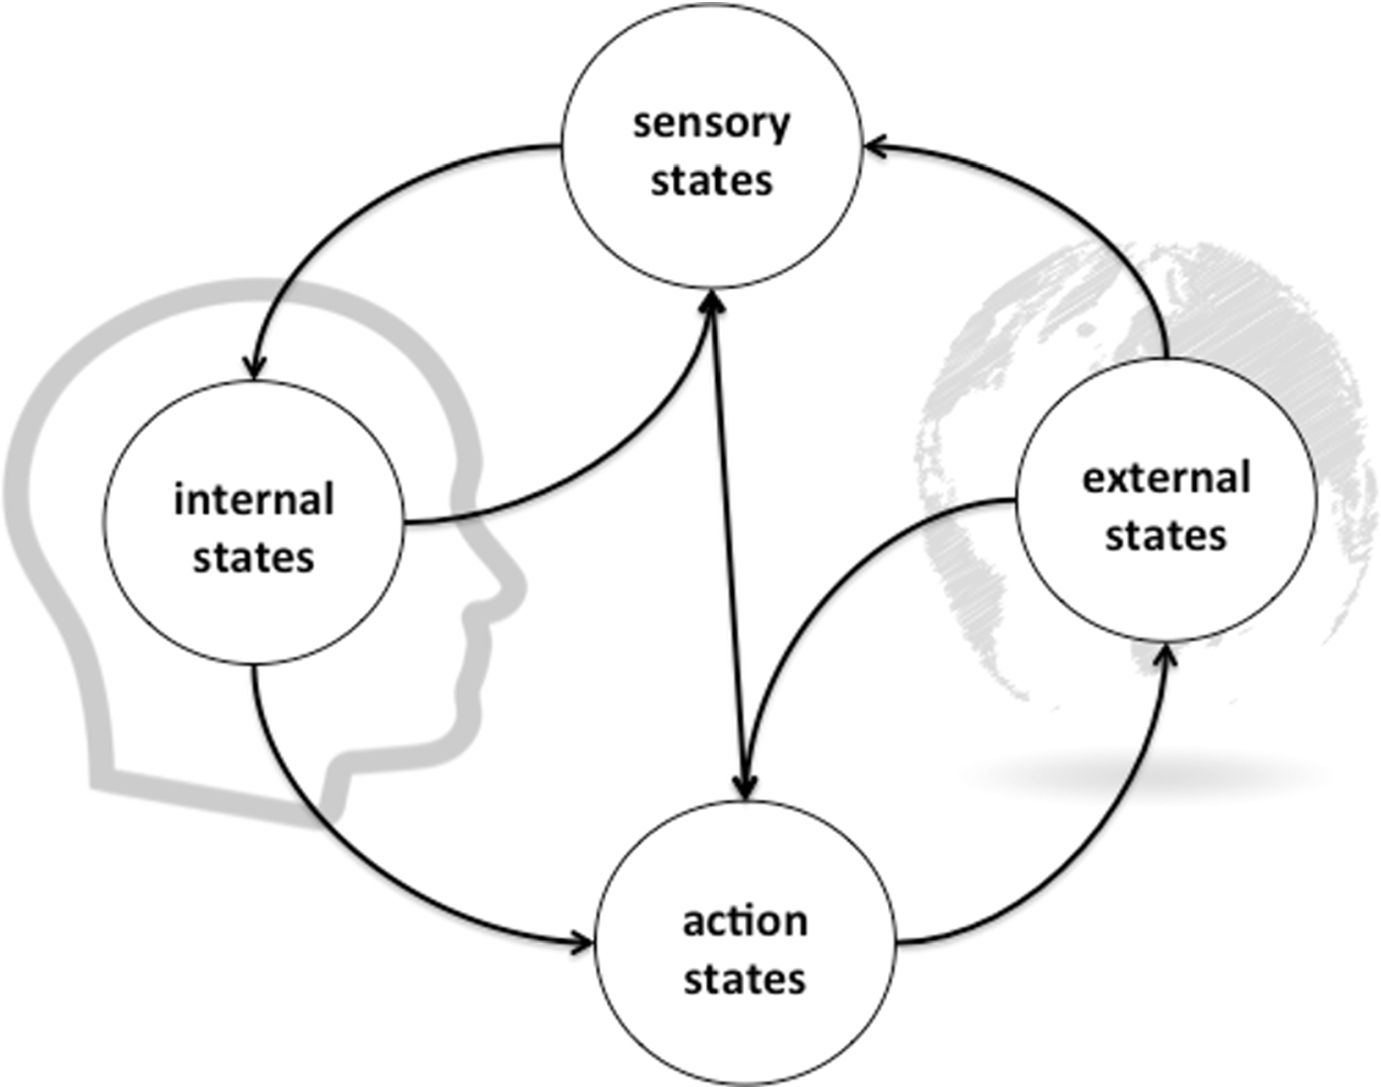
\includegraphics[width=0.8\textwidth]{FEP}
  \caption{A depiction of the various sets of states and their relationships in the FEP}
  \label{fig:FEP}
\end{figure}

The primary appeal of the Active Inference formulation of intelligence/adaptive Behaviour is twofold. First, it unifies the study of action, perception and planning under a single imperative, that of minimizing variational - or expected - free energy. This is an efficient formulation of these problems, since one need only address a single methodological principle instead of three. Parsimony of this kind is always desirable in any scientific theory - all things being equal - since the generality of a theory is very often a good measure of its predictive power.  

Secondly, Active Inference addresses a problem which has plagued value-function formulations of adaptivity since their inception. This is the issue of sample-efficiency and of learning in the presence of sparse rewards: \textcite{RLflawed} and \textcite{RL-Real-World-Challenges}. If all that is available to the agent for generating actions or policies is a value function, mapping states and/or actions to an extrinsic reward signal, it is necessary to observe a great deal many state or state-action par is to learn the optimal mapping from state/state-action to reward signal. For problems with large state-action spaces, this presents a significant challenge to such methods. Active Inference eschews this issue by placing ``information-seeking'' on the same footing as value maximization and hence drives the agent to dynamically trade-off attention between these two goals. 

Use the ``colored room'' example?


\textcolor{red}{Active inference is interesting because of its promise to be such a general method and indeed owing to a growing body of empirical research to suggest that free-energy minimization is what the brain is doing - I have citations for this. Since the brain is thought to be the seat of "natural" intelligence, evidence attesting to the brain's function as a "free-energy minimizing machine" must surely be of interest to we who are concerned with generating instances of intelligence, artificially.}

This is fine, though try to avoid ``grandiose'' claims. A better approach is to lead with an explanation as to what it is that Active Inference solves and perhaps how it is novel in a useful way. 

Active Inference has typically only been implemented on relatively trivial problem instances, with a small number of states and/or actions, and in a discrete setting. T-maze, saccadic eye movements, examples... The goal of scaling up the method to problems with larger state and/or action spaces, such as in the continuous case, is an open problem, and one that would afford X, Y and Z valuable capabilities.  

\subsection{Active Inference: Key Concepts} 
\textbf{Provide brief overview of key concepts and theories to be discussed in the review}

Things that will some elaboration, or at least a definition:

\begin{enumerate}
	\item Free Energy principle
	\item Bayesian Inference
	\item Variational Inference
	\item Variational Free Energy
	\item Expected Free Energy
	\item Model-Based vs Model-Free Methods - not sure if this is necessary
	\item Factor Graphs and Message Passing
	\item Policy (Reinforcement Learning vs Active Inference framing)
	\item Amortized Inference
\end{enumerate}

There are too many here to do full justice in the manner you desire. Maintain a glossary of key terms, in addition.

\subsection{Overview of Research Direction}

\textbf{Perhaps also reiterate the research question? - certainly later, after the body of the review.}

The central aim of my proposed research topic is twofold. The first constituent aim is to investigate the relative merits/demerits of active inference as a real-world control and optimization strategy, against reinforcement learning baselines. I propose to investigate this by framing the question of real-world suitability in terms of the approach's ability to afford fast and reliable solutions in noisy, uncertain or partially observable environments. the subsequent active inference agents I develop will be compared to Reinforcement Learning baselines. 

The second aim concerns the potential for ``scaling up'' Active Inference methods to continuous and/or higher-dimensional state-spaces. This is a natural corollary to the first aim, since if we are interested in the suitability of Active Inference as a real-world control and optimization technique, it is not enough to simply determine if it can favorably compare to an established method in the noisy case. Since the real-world tasks of interest are overwhelmingly characterized by a high degree of dimensionality, it is necessary to investigate the performance of Active inference in high-dimensional settings.  

Thus are the central questions raised in this Thesis:

\begin{itemize}
\item Are Active Inference agents more robust to noisy observations and non-stationarity than a comparable RL baseline?
\item What are the most promising avenues of investigation in the attempt to scale up active inference to larger problem instances? 
\end{itemize} 

\section{Previous Work}

This thesis aims to investigate two distinct approaches to the affordance of the use of active inference methods in larger problem instances than have been practical to tackle with the method. In addition, the investigation is also concerned with unearthing any potentially systematic advantages the method might have, compared to reinforcement learning, with respect to model robustness in the presence of observation noise.

Attempts to address these twin issues; scaling active inference to larger problem instances and investigating its robustness as compared with more standard methods, have already begun to appear in the literature, though these endeavors are still very much in their infancy. 

\textcite{Emperical-Eval-AIF-Multi-Arm-Bandits} implemented an Active Inference agent for the multi-armed bandit problem, in the stationary and non-stationary case. In the stationary case, this agent Active did not perform as well as a special purpose, state-of-the-art Bayesian UCB algorithm. However in the non-stationary case, the Active Inference agent outperformed the UCB agent. While this implementation was conducted over a small, discrete state-action space, the results plausibly suggest that Active Inference would be an effective means of robust inference and control in a higher-dimensional or continuous problem.  

more on the robustness issues goes here...

\subsection{Factor Graphs and Message Passing Methods}

A particularly novel approach that has enjoyed some success as of late, casts the problem of inference as a species of message passing updates on a Forney factor graph: \textcite{Factor-Graph-Approach-Automated-Design-Bayesian-Algos}, \textcite{Simulating-AIF-By-Message-Passing}, \textcite{Factor-Graph-Desc-Deep-Temp-AIF} and \textcite{Reactive-MP}. 

In this framework, the agent's generative model is constructed in such a was as to instantiate a Forney or ``Normal'' factor graph: \textcite{Codes-on-Graphs}. Free Energy minimization is then cast as a process of message passing over this factor graph. Various message passing algorithms exist, such as Belief Propagation and Variational Message Passing. This message passing scheme greatly reduces the number of terms over which it is necessary to sum, when computing the approximate marginal and posterior distributions; affording much more efficient inference and a great potential for scaling up to larger state-action spaces. Indeed, this method does not make use of any approximation by means of a sampling procedure. Since this method relies upon a particular schedule of message-passing update rules on the underlying factor graph, all functions used need to be invertible and an inference is performed via a closed form update where the prior and likelihood distributions must be conjugate. The model passes around full distributions instead of mere samples. This results in a very fast and efficient implementation - when applicable, but the issue is that it is not a completely generic method as of yet, owing to the many assumptions as to the model structure just enumerated. 

\subsection{Sampling Based Approximation Methods}

A more standard approach that has seen a comparatively greater deal of attention is that of using deep neural network function approximators to either parameterize the distributions of interest, or to afford an efficient means of sampling these distributions. This affords approximate inference. Indeed this "genre" of approach has already seen great success in scaling reinforcement learning methods to larger state-action spaces: \textcite{Async-Methods-Deep-RL}, \textcite{ATARI-Deep-RL}, other citations needed and available.

See: \textcite{Deep-AIF}, \textcite{Applications-of-FEP-Machine-Learning-Neuroscience}, \textcite{Deep-AIF-As-Var-Policy-Grad}, \textcite{Reinforcement-Learning-Through-AIF} and \textcite{Bayesian-Policy-Selection-Using-AIF}. 

Of particular interest are: \textcite{Scaling-AIF}, \textcite{Bayesian-Policy-Selection-Using-AIF} and \textcite{Contrastive-AIF}. The former makes use of amortized inference, in the form of neural network function approximators to parameterize the relevant distributions. Free Energy minimization is then performed with respect to the function approximators. In addition, the free energy functional is amortized over the training data. This affords several advantages. For example, the number of parameters remains constant with respect to the size of the data and inference can be achieved via a single forward pass through the network. This contrasts with the iterative approach, where the VFE must be scored for every sample, individually. The resulting algorithm was able to explore a much greater proportion of the state space in a simple stationary environment, in comparison with two Reinforcement Learning baseline agents. In addition, the agent was able to learn to control the continuous inverted pendulum task with a far greater sample efficiency than the baseline agents. Although the approach offered in \textcite{Scaling-AIF} is promising, its analysis was restricted in every case to fully observable environments. This potentially sold the implementaon short, since the partially observable domain is the more "natural" problem instance for which active inference was conceived as a solution strategy. Active Inference has a built-in drive to effect uncertainty reduction, this is not so with standard reinforcement learning, for which only ad-hoc strategies exist to afford the same sort of epistemic drive that exists in active inference. This is a salient point of departure between active inference and reinforcement learning, since both already implement strategies for realizing pragmatic value. 

Pragmatic value is encoded as the sum of discounted reward across time, in the case of reinforcement learning. In the case of active inference, the drive to realize pragmatic value is afforded by the choice of action/s that realize the agent's prior preferences. The realization of prior preferences in active inference is analogous to maximizing the reward signal in reinforcement learning. However there is no analogous process for a drive to realize epistemic value, going from active inference to reinforcement learning, at least not without some aforementioned ad-hoc contrivance of the reward signal. 

Lastly, the approach of \textcite{Contrastive-AIF}, implemented a contrastive method for their Active Inference agent, which significantly reduced the computational burden of learning the parameters for the generative model and planning future actions. This method performed substantially better than the usual, likelihood-based ``reconstructive'' means of implementing Active Inference and it was also computationally cheaper to train. Importantly, this method offered a unique way to afford increased model-robustness in the face of environmental distractors. 


\section{Gaps in Literature}
Though there has been much focus on the implementation of active inference methods for small, discrete state-action spaces: \textcite{Applications-of-FEP-Machine-Learning-Neuroscience}, \textcite{AIF-Discrete-Action-Spaces-Synthesis}, \textcite{Step-by-Step-Tutorial-AIF-Empirical-Data}, \textcite{Relationship-Dynamic-Programming-AIF} and \textcite{AIF-Epistemic-Value}. The method is not currently viable for practical use in larger or continuous state-action spaces, for which it is necessary to plan future actions over some time horizon. Owing to the relatively small size of the state-action spaces in which active inference has historically been implemented, it has been possible to simply evaluate the expected free energy of all possible actions over the specified time horizon. This owes primarily to the issue of evaluating the expected free energy, which is the expectation of the Variational free energy evaluated for future actions over some time horizon: \textcite{Message-Passing-Perspective-Planning-Under-AIF} and \textcite{Bayesian-Policy-Selection-Using-AIF}. 

Unfortunately, enumerating all possible action-trajectories over the specified time horizon does not scale well to problems with larger state-action spaces
and/or longer time horizons. Hence we can now specify exactly what it is that the problem of ``scaling'' is supposed to be. 

Let $S$ be a solution technique. Let $P_1$ and $P_2$ be problem instances of the same type. Let $X$ and $Y$ be the solution spaces for $P_1$ and $P_2$ (respectfully), where $|X| << |Y|$. Suppose the solution technique $S$ affords an adequate solution to problem instance $P_1$, in the sense that the solution is both adequate for the task at hand and $S$ found the solution in an adequate amount of time, consuming an acceptable amount of computational resources. 

$S$ will be is said to scale (or scale well) to problem instance $P_2$, if $S$ can generate a solution to $P_2$, in an acceptable amount of time, while consuming an acceptable amount of computational resources. In other words, the cost associated with generating the solution to $P_2$ does not outweigh the utility of being able to generate the solution to $P_2$, $S$ is a ``viable'' solution technique for instance $P_2$. 

Evaluating all possible trajectories in a problem instance's state-action space, scales exponentially with the size of the state-action space: \textcite{Applications-of-FEP-Machine-Learning-Neuroscience}. For large state-action spaces, evaluating all possible action trajectories quickly becomes an ``unviable'' solution technique.

\section{Research Aims}

I thought I'd reiterate the research questions here and aim to clarify what exactly it is that I seek to achieve.

\section{Conclusion}

Here I think I'll reiterate why this problem of scaling active inference is important at all and suggest potential implications for being able to make some headway in on this problem. 


\section{Overall Plan/Scaffold}

This is simply the list of papers I intend on citing. I won't be able to cite all of them but I think it's best to write what I think I need to write and then cull.

Introductory/Context-Affording papers:
\begin{enumerate}
	\item ``The free-energy principle: a rough guide to the brain?'': \textcite{FEP-Rough-Guide-Brain}
	\item ``Reinforcement Learning: An Introduction'': \textcite{Reinforcement-Learning-An-Introduction}
	\item ``Action and behavior: a free-energy formulation'': \textcite{Action-Behaviour-FE}
	\item ``Mastering the game of Go without human knowledge'': \textcite{Mastering-Go-Without-Human-Knowledge}

	\item Issue scaling AIF ``Active inference on discrete state-spaces: A synthesis'': \textcite{AIF-Discrete-Action-Spaces-Synthesis}
	\item Issue scaling AIF ``A step-by-step tutorial on active inference and its application to empirical data'': \textcite{Step-by-Step-Tutorial-AIF-Empirical-Data}
	\item Issue scaling AIF ``Applications of the FEP to ML and Neuroscience'': \textcite{Applications-of-FEP-Machine-Learning-Neuroscience}

	\item Contemporary RL Method ``Asynchronous Methods for Deep Reinforcement Learning'': \textcite{Async-Methods-Deep-RL}
	\item Contemporary RL Method ``Playing Atari with Deep Reinforcement Learning'': \textcite{ATARI-Deep-RL}

	\item ``Reinforcement Learning or Active Inference?'': \textcite{RL-or-AIF}
	\item ``The FEP for action and perception a mathematical review'': \textcite{FEP-Mathematical-Review}
	\item ``The Bayesian brain: the role of uncertainty in neural coding and computation'': \textcite{The-Bayesian-Brain}
	\item ``An empirical evaluation of active inference in multi-armed bandits'': \textcite{Emperical-Eval-AIF-Multi-Arm-Bandits}
	% \item "": \textcite{}
\end{enumerate}

Neural Network Approximators:
\begin{enumerate}
	\item ``Applications of the FEP to ML and Neuroscience'': \textcite{Applications-of-FEP-Machine-Learning-Neuroscience}
	\item ``Deep Active Inference'': \textcite{Deep-AIF}
	\item ``Deep Active Inference as Variational Policy Gradients'': \textcite{Deep-AIF-As-Var-Policy-Grad}
	\item ``Scaling Active Inference'': \textcite{Scaling-AIF}
	\item ``Reinforcement Learning Through Active Inference'': \textcite{Reinforcement-Learning-Through-AIF}
	\item ``Bayesian Policy Selection Using Active Inference'': \textcite{Bayesian-Policy-Selection-Using-AIF}
	\item ``Contrastive Active Inference'': \textcite{Contrastive-AIF}
\end{enumerate}

Factor Graph and Message Passing Implementations
\begin{enumerate}
	\item ``Codes on graphs: normal realizations'': \textcite{Codes-on-Graphs}
	\item ``Simulating Active Inference by Message Passing'': \textcite{Simulating-AIF-By-Message-Passing}
	\item ``Applications of the FEP to ML and Neuroscience'': \textcite{Applications-of-FEP-Machine-Learning-Neuroscience}
	\item ``A factor graph approach to automated design of Bayesian signal processing algorithms'': \textcite{Factor-Graph-Approach-Automated-Design-Bayesian-Algos}
	\item ``Reactive Message Passing for Scalable Bayesian Inference": \textcite{Reactive-MP}
	\item ``A Factor Graph Description of Deep Temporal Active Inference'': \textcite{Factor-Graph-Desc-Deep-Temp-AIF}
	\item ``Deep Active Inference for Partially Observable MDPs'': \textcite{DEEP-AIF-For-POMDPs}
	\item ``Bayesian policy selection using active inference'': \textcite{Bayesian-Policy-Selection-AIF}
\end{enumerate}

Finally, address the specific papers on Scaling that I'll use:
\begin{enumerate}
	\item Sampling/Neural Networks ``Scaling Active Inference'': \textcite{Scaling-AIF}
	\item Sampling?/neural nets? "``Contrastive Active Inference'': \textcite{Contrastive-AIF}
\end{enumerate}

Other Papers:
\begin{enumerate}
	\item Paper: ``The FEP for action and perception a mathematical review'': \textcite{FEP-Mathematical-Review}
	\item paper: ``Simulating Active Inference by Message Passing'': \textcite{Simulating-AIF-By-Message-Passing}
	\item Paper: ``a practical tutorial on Variational Bayes'': \textcite{Practical-Tutorial-Variational-Bayes}
	\item Paper: ``action and behavior, a free energy formulation'': \textcite{Action-Behaviour-FE}
	\item paper: ``A tutorial on the free-energy framework for modelling perception and learning'': \textcite{Tutorial-FEP-Modelling-Perception-Action}
	\item Paper: “A step-by-step tutorial on active inference and its application to empirical data'': \textcite{Step-by-Step-Tutorial-AIF-Empirical-Data}
	\item Paper: ``Scaling Active Inference'': \textcite{Scaling-AIF}
	\item paper: The Cape Town AIF/RL Honours Thesis - not sure if published/if appropriate
	\item PhD Thesis: ``Applications of the FEP to ML and Neuroscience'': \textcite{Applications-of-FEP-Machine-Learning-Neuroscience}
\end{enumerate}

% \bibliographystyle{IEEEtran}
\printbibliography

\end{document}
